\documentclass{article}
\usepackage{geometry}
\geometry{a4paper, top=3cm, bottom=3cm, left=2cm, right=2cm}
\usepackage[utf8]{inputenc}
\usepackage[english]{babel}
\usepackage{hyperref}
\makeindex

\title{Blockchain and Cryptocurrencies}
\author{Riccardo Salvalaggio}
\date{19th of April, 2021}

\usepackage{amssymb}
\usepackage{amsmath}
\usepackage{txfonts}
\usepackage{mathdots}
\usepackage[classicReIm]{kpfonts}
\usepackage{graphicx}

\begin{document}

\maketitle
\newpage
\tableofcontents
\newpage

\section{Introduction}
\textbf{Ledger: }record of transaction history, centralized, unforgeable.\\
\textbf{Blockchain: }Decentralized ledger, replicated, need of consensus (blocks because updating at each transaction would be too expensive).\\
\textbf{Cryptocurrency: }digital money, cryptographic means, rely on blockchain.\\
\textbf{Non-monetary Uses: DApps} - Decentralized Apps - Smart contracts: storing and executing programs on the blockchain. (e.g.: crypto assets, smart property, voting).\\



\section{Money}
Money formalizes the accounting, keeps track of global favor-granting and is useful as memory.
\subsection{Payment Systems}
A payment system is based \textbf{on representation of money, creation of it, and transfer of ownership}.
\textbf{Cash: }physical, has storage and transport drawbacks.\\
\textbf{Electronic: }mainly digital, physical token required (e.g.: credit card), book money, centralized point of failure.\\
\textbf{Blockchain-based: }no physical, algorithmic creation, decentralized consensus.\\
\subsection{Monetary unit}
The need of a unit emerges from social processes and ease of interchanging. \textbf{Functions: }mean of exchange (w/o money too much exchanging), unit of accounting (allows an interpretation of prices, to compare valuation of goods and in order to have market transparency)and value storage (possibility of save in order to make larger investments).\\
\textbf{Properties: }durability, transferability, divisibility, homogeneity, verifiability, stability, scarcity.
\subsection{Monetary equivalent}
Why money has value? Fundamental value (material), payment promise (what you can buy with that), speculation (based on demand for the object and possibility of variation).\\
\subsubsection{Fiat Money}
No fundamental value, no payment promise, value entirely based on expectation (no bounds). Most currencies now are Fiat, the value is maintained by a central bank and have legal tender.
\subsection{Monetary Control Structures}
Two modes of money creation: \textbf{Competitive: } (everybody can, limit: production < market value) two possible scenario: gold mining, constant low creation cost, \textbf{Monopolized: } (restricted to government agencies) artificially limited.
\subsubsection{Creation by Banks}
The central bank creates money by loaning to corporate banks. Temporary loans help regulate the money supply. Corporate banks can create money by lending or deposit currency" (to private customers and businesses) that is not backed by legal tender. If all customers withdraws legal tender the bank goes bankrupt.
\subsection{Money representations}
\textbf{Physical}: physical ownership, easy to use. Bound to location, integrity, divisibility.\\
\textbf{Virtual}: digital representation of a value not bounded to a real currency. It is nevertheless accepted as a means of payment and can be transmitted, stored and traded. Ownership achieved by cryptographic certificates.\subsection{Transaction processing}
\textbf{Conditions:} Capability: transactions can be started and value can be transferred, Legitimacy: only by the owner, Consensus: process to determine the current balance of everyone.

\section{Basic Tools}
\subsection{Blockchain}
A blockchain is a growing list of records, called blocks, that are linked using cryptography. Each block contains a cryptographic hash of the previous block, a timestamp, and transaction data.\\
A transaction is a movement of a monetary item. Transaction history is public, so everyone can know your balance and check every transaction. It's alright unless the history can be rewritten/faked.

\subsection{Cryptographic Hash Functions}
In the Blockchain, every block consists of the text of the transactions and the hash of the preceding block.\\
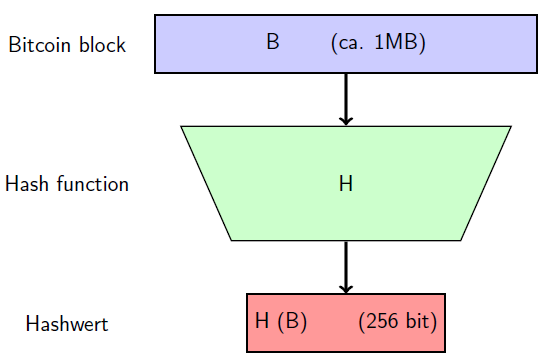
\includegraphics[scale=0.6]{1.png}\\
A hash function is a mapping h : B* -\textgreater B at n, for some n \textgreater 0. B = ${0,1}$.\\
A compression function is a mapping h : B at m -\textgreater B at n, for some m \textgreater  n \textgreater 0.\\
Function h is a one-way function (or preimage resistant) if, given some s in Bn, it is practically impossible to find a preimage x in D such that h(x) = s.\\
A collision of h is a pair (x; x0) with x != x0 in D such that h(x) = h(x0).\\
A function h is second preimage resistant (weakly collision resistant) if, given some x in D, it is practically impossible to find x0 such that (x; x0) is a collision of h.\\
A function h is collision resistant if it is practically impossible to find a collision (x; x0) of h.\\
Any second preimage resistant function h is also one-way.\\
Any collision resistant function is also second preimage resistant.(See proofs)\\

\subsubsection{Find a collision}
Bitcoin uses SHA-256 so output is B at 256. To find a collision you need more time than universe age. It is practially impossible to nd a collision (x; x0) for h.\\
Birthday Paradox: we need to do just ~N/2 in order ot have 0.5 probability of exploiting the correct answer.

\subsubsection{Hash from Compression}
Merkle-Damgaard procedure: Let f : Bm -\textgreater Bn be a compression function and let r = m - n \textgreater=  2. The goal is to construct a hash function h : B* -\textgreater Bn from f .\\ Preprocessing: becomes b'||0 at k||x||0 at r of length t*r.\\\\
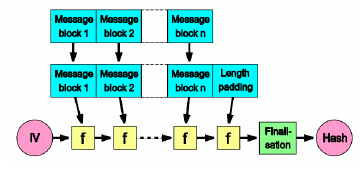
\includegraphics[scale=0.8]{2.png}\\\\
If f is collision resistant, then the Merkle-Damgaard construction yields a function h that is also collision resistant.\\
\subsubsection{Properties and Applications}
Use of MAC for integrity of Data. \\
- Hiding: consequence of using a one-way. Small inputs can be a problem. To solve: Instead of computing h(x), compute h(rkx) where r is a suitably chosen random number.\\
- Commitment scheme (MAC scheme): commit and verification. Reqs: Hiding (given com it is infeasible to find msg) Binding (it is infeasible two find two mesages tht return same commit). To enforce, use nonce, number used once: it add perturbation.\\
- Def. Puzzle friendly: if for every possible n-bit output value and every k
chosen from a distribution with high min-entropy, then it is infeasible to and x such that h(k||x) = y in time significantly less than 2 at n.\\
SHA-256 is defined via the Merkle-Damgaard construction from a compression function the compression function is designed such that flipping a bit in the input changes at least 50$\%$ of the bits in the output. Not know to be compromised, but successors exist since 2012: SHA-3 (Keccak).

\section{Cryptography and Digital Signatures}
\subsection{Public key cryptography}
- Symmetric encryption: Encode, Decode. \textbf{Decode(k,encode(k,m)) = m.}\\
Partners needs same key, if it is exposed, confidentiality is compromised.\\
- Asymmetric encryption: Pair of different keys: Pub$\_$K, Pri$\_$K. Public key is freely shared, the private is known only by the owner. Asymmetric is more expensive than symmetric, so most of the times is only used for key exchanging.\\
\textbf{Decode(Pri$\_$K,encode(Pub$\_$k,m)) = m.} It is a one-way encryption.\\\\
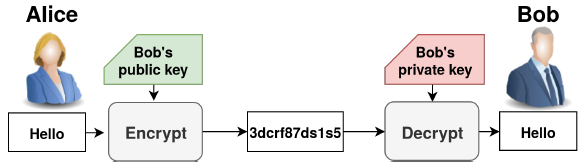
\includegraphics[scale=0.8]{3.png}\\\\
- Cryptosystem: Key pair, keygenerator, encode, decode (polynomial time algorithm).\\

\subsubsection{RSA}
Choose two primes p,q: n= pq of k bits.\\
Choose 1<e<(p-1)(q-1): e is coprime with (p-1)(q-1).\\
Choose 1<d<(p-1)(q-1): de=1mod(p-1)(q-1). (thanks to EEA)\\
Pub$\_$key = (n,e), Pri$\_$key = d.\\\\
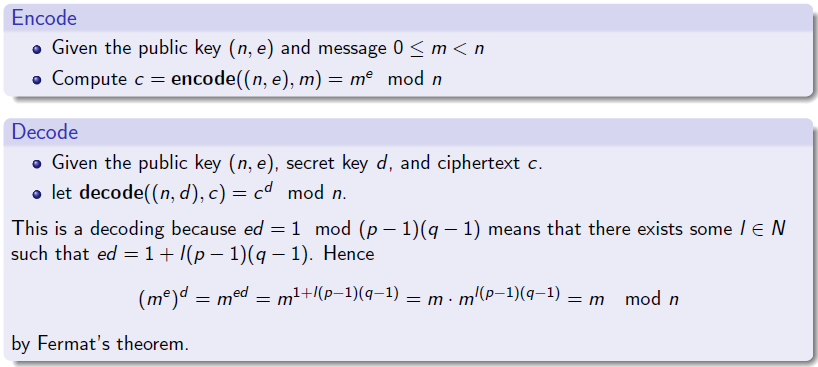
\includegraphics[scale=0.8]{4.png}\\\\
Bitcoin uses a different scheme based on Elliptic curves.\\

\subsection{Digital Signatures}
Signature is a handwritten depiction of someone's name, nickname etc.\\
\textbf{Functions:} proof that signer has seen the content of the document, integrity of the document, signature has to be difficult to forge, but easy to verify.\\
Same mechanism of Public-key cryptography but sign with private and decrypt with public, so everyone can decrypt but only the owner can sign.\\\\
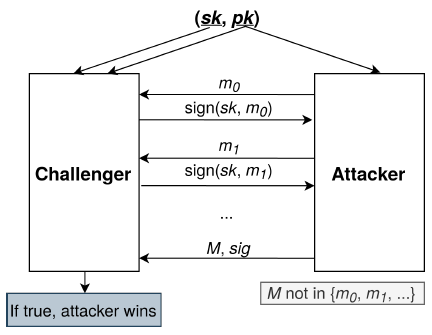
\includegraphics[scale=0.8]{5.png}\\\\
- Practical concerns: many algorithms are probabilistic, limit on message size (possible solution, sign the hash).\\
Bitcoin uses ECDSA (Elliptic Curve Digital Signature Algorithm) that provide 128 bits: Pri$\_$K = 256 bits, Pub$\_$K = 512 bits (compressed 257 bits), m$\_$size = 256 bits, signature = 512 bits.\\

\subsection{Identities}
Identity consists of a pair (Pri,Pub).\\
Decentralized Identity Management: new identities can be created at any time, good randomness source is required, no need for central user registry, but transactions may reveal behaviour and connections.\\



\end{document}
